\documentclass{article}
\usepackage{tikz}

\begin{document}

\begin{center}
    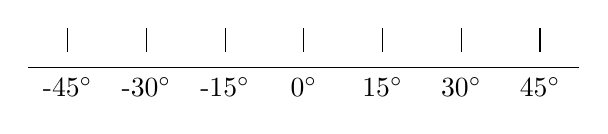
\begin{tikzpicture}
        % Achse
        \draw[-] (-3.5,0) -- (3.5,0);

        % Striche und Beschriftung in 15°-Schritten
        \foreach \x in {-45,-30,-15,0,15,30,45} {
            \draw (\x/15,0.2) -- (\x/15,0.5); % Striche
            \node[below] at (\x/15,0) {\x$^\circ$}; % Zahlen darunter
        }
    \end{tikzpicture}
\end{center}

\end{document}

